\subsection{Description}
This mono effect creates adds a futuristic sweeping sound to a sample track. This is done using a series of all-pass filters which maintain the magnitude of a signal while applying a nonlinear phase shift. In order to create a sweeping effect, the center frequency of each all-pass filter is varied with an LFO.

\subsection{Applications}
Typically, phasers are used by guitarists to create an electronic or unnatural sound for tracks that are meant to sound futuristic or ethereal.

\subsection{Principles of Operation}
A basic phaser is composed of a series of all-pass IIR filters. However, a single filter alone cannot create the notches in the output spectrum that are characteristic of phasers. In an analog implementation, four first order filters or two second order filters. Each all-pass filter maintains the magnitude of the signal, but it applies a nonlinear phase shift to the input phase. The overall output phase is the sum of the phase shift added by each filter. This filtered signal is then amplified and added to the original signal. This create multiple notches in the output spectrum as seen in Figure \ref{fig:phaser-spectrum}. Each notch represents destructive interference between the filtered signal and original signal.
\begin{figure}[ht]
    \centering
    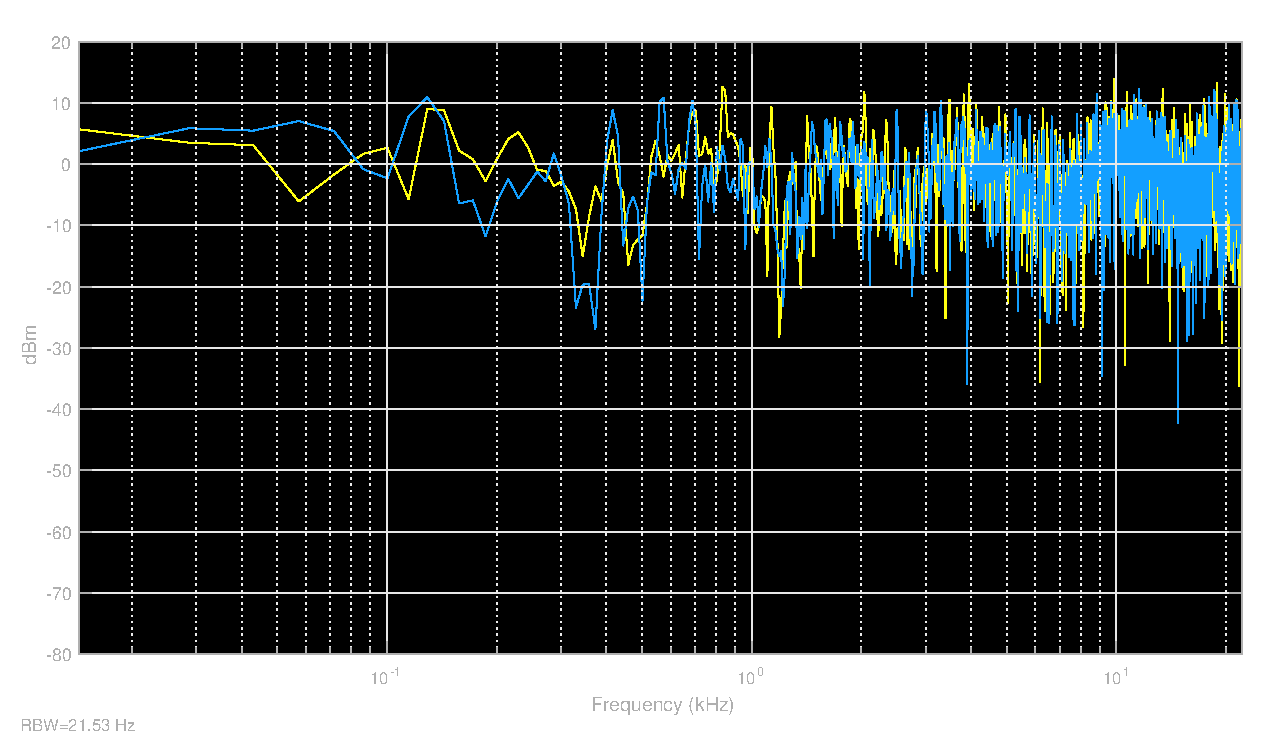
\includegraphics[scale=0.5]{phaser-spectrum.eps}
    \caption{Output Spectrum of a Phaser Effect}
    \label{fig:phaser-spectrum}
\end{figure}
In order to move the notches, the center frequencies of each filter is varied using an LFO. Each filter has the same center frequency. The LFO output is given by Equation \ref{eq:phser-lfo} and shown in Figure \ref{fig:phaser-lfo-waveform}.
\begin{equation}
    f_c[n] = f_{min}\left(\frac{f_{max}}{f_{min}}\right)^{triangle(\omega_{LFO} n)}
    \label{eq:phser-lfo}
\end{equation}
\begin{figure}[ht]
    \centering
    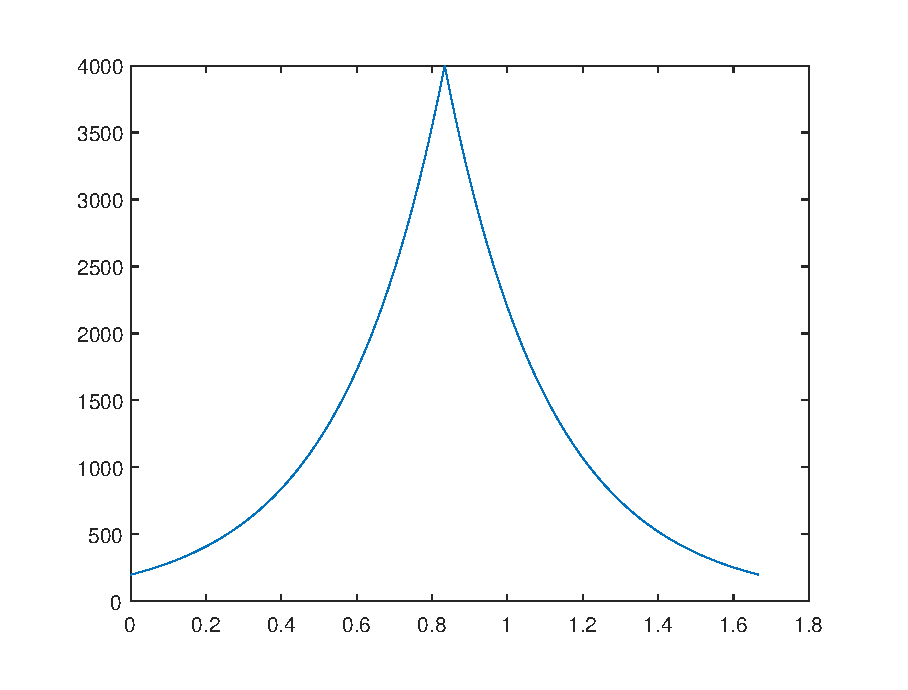
\includegraphics[scale=0.5]{phaser-lfo-waveform.eps}
    \caption{Phaser LFO Output Between 200 Hz and 4000 Hz}
    \label{fig:phaser-lfo-waveform}
\end{figure}
In order to improve the $Q$ of the all-pass filters, a feedback path can be added. The full block diagram with feedback is shown in Figure \ref{fig:phaser-block-diagram}.
\begin{figure}[ht]
    \centering
    \includegraphics[scale=0.3]{phaser-block-diagram.png}
    \caption{Phaser Block Diagram with Three Allpass Filters}
    \label{fig:phaser-block-diagram}
\end{figure}

\subsection{Implementation}
Our implementation for phaser is unique, because it uses the STFT to move the time domain input signal into the frequency domain, then apply the appropriate phase shift with simple addition, then move the filtered spectrum back into the time domain. Typically, a phaser implemented in \href{run:../phaser.m}{MATLAB} would make use of the biquad filter command instead of using an STFT and frequency domain phase processing.

\subsection{Demo and Discussion}
The effect is most easily heard in \href{run:../OutputAudio/phaser_noise_{depth=1}{fc_min=200Hz}{fc_max=4000Hz}{f_LFO=0.2Hz}.wav}{output for colored noise}. However, this is not very interesting. Applying the effect to \href{run:../InputAudio/11-014 Guitar Src.wav}{an original guitar sample} results in a more pleasing \href{run:../OutputAudio/phaser_11-014 Guitar Src_{depth=1}{fc_min=200Hz}{fc_max=4000Hz}{f_LFO=0.2Hz}.wav}{output}. If a not so subtle effect is desired, then the LFO frequency can be increased from 0.2 Hz to \href{run:../OutputAudio/phaser_11-014 Guitar Src_{depth=1}{fc_min=200Hz}{fc_max=4000Hz}{f_LFO=0.8Hz}.wav}{0.8 Hz} or even \href{run:../OutputAudio/phaser_11-014 Guitar Src_{depth=1}{fc_min=200Hz}{fc_max=4000Hz}{f_LFO=1.2Hz}.wav}{1.2 Hz}. The effect can also be applied with \href{run:../OutputAudio/phaser_nofb_11-014 Guitar Src_{depth=1}{fc_min=200Hz}{fc_max=4000Hz}{f_LFO=0.2Hz}.wav}{no feedback}, though the differences are less subtle.

\subsection{Further Exploration}
You can check out an obvious use of phaser in Billy Joel's \href{https://www.youtube.com/watch?v=tJWM5FmZyqU}{Just the Way You Are}. A more subtle use of the effect can be heard in Led Zeppelin's \href{https://www.youtube.com/watch?v=ZDwotNLyz10}{Kashmir}. It may not be clear at first, but if you listen to the drums, especially the crash of the symbols, you can hear a soft phaser being applied.